% !TEX encoding = UTF-8
% !TEX TS-program = pdflatex
% !TEX root = ../Lahmer_Abdelilah_tesi.tex
% !TEX spellcheck = it-IT

%**************************************************************
\chapter{Il progetto di Stage}

\section{Pianificazione del lavoro}
%In questo inizio di sezione parlerò della pianificazione del lavoro per il progetto di stage in fatto di tempistiche.
Per raggiungere gli obiettivi pianificati nel piano di stage e rispettare i requisiti minimi imposti dall'Università, io e il tutor aziendale abbiamo previsto 304 ore di lavoro, distribuite in circa 8 settimane da 40 ore ciascuna. Ho iniziato lo stage il 17 Maggio 2017 e terminato il 10 Luglio 2017, rimanendo in linea con quanto pianificato inizialmente, senza incorrere in particolari differimenti da quanto programmato.

\subsection{Definizione del piano di lavoro}
%In questa sottosezione parlerò della pianificazione del lavoro per il progetto di stage riportando i dati dal piano di lavoro con la programmazione delle ore da dedicare a ciascuna attività.
	Nei giorni immediatamente precedenti l'inizio dello stage mi sono recato in sede Sopra Steria e ho redatto il Piano di Lavoro, con conseguente revisione del tutor aziendale. In questo documento ho definito gli obiettivi e la pianificazione delle attività, assegnando ad ognuna una tempistica in ore e suddividendo l'intero percorso di stage in tre fasi. Ho specificato inoltre le modalità di interazione col tutor e una previsione delle competenze che sarei andato ad acquisire.\\

Tramite il Piano di Lavoro e la pianificazione dettagliata in esso avrei potuto infatti verificare l'effettivo allineamento tra il lavoro svolto e il lavoro pianificato man mano che il percorso di stage volgeva al termine.\\
	
Settimanalmente inoltre aggiornavo il mio tutor interno sulla mia situazione in relazione alla pianificazione, riportando eventuali scostamenti dal Piano di Lavoro. \\

\newpage

	Le fasi individuate in tale documento sono state:
	
	\begin{itemize}
		\item \textbf{FASE 1 - Formazione tecnica}: durante questa prima fase del percorso formativo era prevista l'introduzione alle modalità di approccio alla programmazione tramite dei corsi a seconda dell'ambiente di sviluppo, tecnologie e linguaggi di programmazione da utilizzare; in particolare era previsto: 
			\begin{itemize}
				\item lo studio e utilizzo dell'ambiente di sviluppo mainframe;
				\item lo studio dei concetti fondamentali del linguaggio di programmazione COBOL\glossario;
				\item lo studio delle modalità di interazione con database DB2;
				\item lo sviluppo di semplici programmi nell'ambito dell'applicazione realizzata da Sopra Steria.
			\end{itemize}
		\item \textbf{FASE 2 - Formazione funzionale}: durante questa seconda fase del percorso formativo era prevista l'introduzione alla metodologia di operatività in ambito funzionale, iniziando a lavorare a stretto contatto con il resto del team della \textit{Business Unit} addetta ai Servizi Finanziari. Erano previste infatti attività di formazione di carattere funzionale in ambito bancario, apprendendo la modalità di collegamento tra quella che è la parte funzionale del sistema con la parte tecnica, introdotta nella FASE 1; in particolare era previsto: 
			\begin{itemize}
				\item lo studio e utilizzo del sistema sviluppato dall'azienda, ovvero ELISE\glossario;
				\item lo studio e utilizzo della parte relativa alla funzionalità di “finanziamenti in Pool\footnote{I finanziamenti in Pool in ambito bancario rappresentano quelli che vengono denominati anche \textit{prestiti sindacati}, sono erogati da un insieme di banche a favore di un'impresa. Scopo di tale raggruppamento è la ripartizione del rischio e dello sforzo di finanziamento.}” all'interno di ELISE;
				\item lo studio delle modalità di trasformazione dei concetti funzionali in tecnici.
			\end{itemize}
		
		\item \textbf{FASE 3 - Analisi tecnica e funzionale modulo “Pool”}: In questa ultima e terza fase del percorso formativo era previsto lo studio della parte tecnica e funzionale di uno dei moduli dell'applicazione orientata ai finanziamenti realizzata da Sopra Steria, ovvero il modulo “Pool”. Era previsto inoltre lo sviluppo in linguaggio COBOL di quelle che sarebbero state le funzionalità studiate ed analizzate nel documento funzionale e tecnico.% In particolare in questa fase del percorso di stage erano previsti:
%			\begin{itemize}
%				\item lo studio e l'analisi del modulo;
%				\item la progettazione dell'analisi funzionale;
%				\item la redazione dell'analisi Funzionale e Tecnica del modulo.
%			\end{itemize}

	\end{itemize}
\leavevmode	\newline

%\newpage
		\begin{center}
		  \bgroup
		  \def\arraystretch{1.4}
		   \setlength\arrayrulewidth{0.6pt}
		   \begin{longtable}{ | p{2.61cm} | p{9cm} |} \hline
		   %\begin{longtable}{ | p{2.5cm} | p{0.5cm} | p{9cm} |} \hline
		   
		    %\cellcolor[gray]{0.9} \textbf{Durata in ore} & \cellcolor[gray]{0.9} & \cellcolor[gray]{0.9} \textbf{Descrizione dell'attività} \\ \hline
		    
		    \cellcolor[gray]{0.9} \textbf{Durata in ore} &  \cellcolor[gray]{0.9} \textbf{Descrizione dell'attività} \\ \hline


			76 	& FASE 1: FORMAZIONE TECNICA \\ \hline

			\tab \tab 24 & Formazione ambiente di sviluppo Mainframe\\
			\cline{2-2}		%\cline{2-2}
			\tab \tab 52 & Formazione linguaggio di programmazione COBOL \\	\hline
			
			76 	& FASE 2: FORMAZIONE FUNZIONALE \\ \hline

			\tab \tab 12 &  Formazione sul sistema sviluppato dall'azienda\\
			\cline{2-2}		%\cline{2-2}
			\tab \tab 12 &   Formazione sulla parte relativa al concetto di “Pool”\\
			\cline{2-2}		%\cline{2-2}
			\tab \tab 52 &  Formazione sulla modalità di trasformazione dei concetti funzionali in tecnici\\	\hline			
			
			152 & FASE 3: ANALISI TECNICA E FUNZIONALE MODULO “POOL” \\ \hline

			\tab \tab 40 &  Analisi modulo \\
			\cline{2-2}		%\cline{2-2}
			\tab \tab 40 &  Progettazione dell'analisi funzionale \\
			\cline{2-2}		%\cline{2-2}
			\tab \tab 72 &   Redazione analisi Funzionale e Tecnica modulo \\	\hline
			
			\caption{Pianificazione delle attività di stage}
			
		    \end{longtable}
		  \egroup
		\end{center}
	
\subsection{Livello di autonomia}
%In questa sottosezione parlerò del livello di autonomia con cui ho svolto lo stage.

	Inizialmente con l'inizio dello stage l'idea era quella di lavorare in un ambiente che mi teneva a stretto contatto con il tutor aziendale, in modo tale da favorire l'interazione e garantire il raggiungimento degli obiettivi prefissati, come da Piano di Lavoro; successivamente però ho scoperto che non sarebbe stato così. Il tutor aziendale infatti, essendo manager di prossimità della sede e facente parte del team degli Analisti Funzionali, era generalmente in trasferte lavorative in sedi distaccate di Sopra Steria oppure dal cliente.\\
	
	Sono stato quindi affiancato da più colleghi della sede per le diverse competenze che dovevo apprendere.\\
	
	Questo tipo di approccio però non è stato positivo; i colleghi a cui sono stato affiancato infatti, soprattutto lato tecnico non sono stati in grado di farmi seguire un percorso di apprendimento proficuo, non avendo particolari metodi di insegnamento oltre ad una visione incompleta dell'architettura dell'applicazione.\\
	
	Questo fattore è stato un deficit rilevante al fine del raggiungimento degli obiettivi prefissati.\\

	Il livello di autonomia che ho raggiunto alla fine del percorso infatti non era sufficiente da poter portare a termine un'attività di sviluppo o analisi in completa indipendenza, necessitavo infatti di saltuarie delucidazioni.\\
	
	La difficoltà di lavoro in modalità autonoma è secondariamente dovuta al fatto che l'ambiente di sviluppo mainframe era a me sconosciuto prima di iniziare l'esperienza di stage, durante il percorso di studi infatti non è mai stato possibile trattatare praticamente questo tipo di contesto. La mancanza di basi di natura economica inoltre hanno sfavorito parzialmente l'autonomia sotto l'aspetto funzionale.

\section{Formazione}
%In questo inizio di sezione farò una panoramica sulla formazione che ho ricevuto, sia quella in ambito teorico-economico sia quella in ambito tecnico.

Le prime due fasi del percorso di stage sono state adibite alla formazione in due ambiti, quello tecnico e quello funzionale. La formazione tecnica si poneva come obiettivo fornire una sufficiente base sul linguaggio di programmazione COBOL e le modalità di sviluppo, utilizzando quest'ultimo, in ambiente mainframe. La formazione funzionale, invece, si poneva come obiettivo quello di apprendimento d'uso di ELISE e dei concetti economici fondamentali utilizzati in esso.

\subsection{Conoscenze economiche acquisite}
%In questa sottosezione parlerò più approfonditamente della formazione in ambito teorico-economico che ho ricevuto e riporterò i macro argomenti trattati, magari con qualche accenno a qualche concetto fondamentale.

Come ho indicato nella sezione dedicata, ELISE è un complesso sistema di gestione di finanziamenti, esso infatti fornisce un ambiente completo che permette il tracciamento di un prestito da quando questo viene istanziato alla sua estinzione. I concetti di natura teorica indispensabili al concepimento degli stati in cui questo può trovarsi e delle funzionalità predisposte dall'applicazione su di esso sono stati oggetto della formazione teorica ricevuta.\\

Di seguito riporterò le più rilevanti nozioni acquisite.

\paragraph{Finanziamento}
Un finanziamento è un rapporto che intercorre tra almeno due soggetti e consiste nella cessione di una somma di denaro con il vincolo della restituzione di capitali di pari valore o maggiori.\\
Gli elementi costitutivi di un finanziamento sono:
	\begin{itemize}
		\item capitale finanziato;
		\item tasso annuo nominale d'interesse (TAN);
		\item tasso annuo effettivo globale (TAEG);
		\item durata del finanziamento;
		\item l'importo, ed eventuali rate e condizioni.	
	\end{itemize}

L'assegnazione di un prestito avviene dopo una serie di controlli preliminari che il mediatore esegue in base alla situazione economica e professionale del soggetto richiedente, esami che gli permettono di valutare la sicurezza evitando sconvenienti situazioni di insolvenza.\footnote{Wikipedia - Prestito (finanza). URL: \url{https://goo.gl/mwp69N}}

\paragraph{Fido}
Un fido bancario, o affidamento, è definito come l'impegno assunto da una banca a mettere una somma a disposizione del cliente, o di assumere per suo conto un'obbligazione nei confronti di un terzo. Un fido bancario può essere concesso sia ad un privato sia ad un'azienda, tuttavia è quest'ultima la categoria che ricorre maggiormente al credito bancario. Gli affidamenti bancari vengono concessi dagli istituti di credito a seguito di una complessa istruttoria che di norma ha ad oggetto sia i profili reddituali che quelli patrimoniali del soggetto richiedente al fine di stabilire la capacità di restituzione del credito concesso (profilo reddituale) e la solidità finanziaria (profilo patrimoniale).\footnote{Wikipedia - Fido bancario. URL: \url{https://goo.gl/49Wwbs}}

\paragraph{Tasso}
In economia, il tasso di interesse effettivo rappresenta la percentuale dell'interesse su un prestito e l'importo della remunerazione spettante al prestatore. Viene espresso come una percentuale per un dato periodo di tempo e indica quanta parte della somma prestata debba essere corrisposta come interesse al termine del tempo considerato o, da un altro punto di vista, indica il costo del denaro. Il debitore, infatti, ricevendo una somma di denaro, si impegna a pagare una somma superiore a quella ricevuta. La differenza costituisce l'interesse, che viene solitamente calcolato in percentuale sulla somma prestata. Tale percentuale costituisce il tasso di interesse. Il tasso d'interesse è variabile anche in funzione della moneta di riferimento, del rischio connesso alla solvibilità del debitore e della lunghezza del periodo di riferimento.\footnote{Wikipedia - Tasso d'interesse. URL: \url{https://goo.gl/AHpfia}}

\paragraph{Piano di ammortamento}
Il piano di ammortamento è un programma di estinzione di debito o di abbassamento o estinzione del capitale di credito. Esistono diversi piani di ammortamento:
	\begin{itemize}
		\item Ammortamento a rate costanti (francese);
		\item Ammortamento con quote capitali costanti (italiano).	
	\end{itemize}
Il piano utilizzato nel sistema bancario italiano è quello alla francese, cioè a rate costanti. Visualizzando il piano di ammortamento ci si accorge che:
	\begin{itemize}
		\item la rata è sempre la stessa (sempre che il tasso non cambi);
		\item la quota interessi è pari al tasso di interesse del periodo per il debito residuo alla fine del periodo precedente;
		\item la quota capitale è la differenza tra rata e quota interessi.\footnote{Wikipedia - Piano di ammortamento. URL: \url{https://goo.gl/vtBdix}}
	\end{itemize}

\paragraph{Finanziamento in Pool}
I prestiti sindacati, conosciuti anche come "finanziamenti in pool", sono erogati da un consorzio di banche (il pool) a favore di un'impresa. Scopo di tale raggruppamento è la ripartizione del rischio e dello sforzo di finanziamento; il pool si scioglie una volta ultimata l'operazione. I prestiti in pool fanno parte di quella categoria di finanziamenti a medio-lungo termine che concedono le banche. I prestiti in pool fanno parte di quella categoria di finanziamenti a medio-lungo termine che concedono le banche. All'interno di un pool si distingue solitamente:
	\begin{itemize}
		\item la banca \textit{arranger} che si assume l'onere dell'organizzazione (in ELISE questa si chiama banca "\textit{rappresentante}");
		\item la banca capofila, (spesso coincide con la banca \textit{arranger}) che coordina dopo la sindacazione;
		\item la banca agente che cura tutti gli aspetti amministrativi dopo l'operatività del prestito;
		\item la banca partecipante che eroga una quota parte del prestito.\footnote{Wikipedia - Prestiti sindacati. URL: \url{https://goo.gl/nQyvFh}}
	\end{itemize}

\subsubsection{ELISE}
%In questa sotto sottosezione descriverò ELISE e spiegherò i suoi scopi e funzionalità principali, collegando infine il tutto con le attività formazione teorico-economiche che ho applicato in essa dopo averle acquisite.

Nella formazione sotto l'aspetto funzionale uno dei principali obiettivi era anche quello di apprendere la modalità d'uso dell'applicazione ambito di progetto, ovvero ELISE, ed acquisire capacità di navigazione all'interno di essa. Quest'attività di apprendimento è strettamente legata alla formazione sui concetti teorico-economici discussi nella sezione precedente.\\

Nel formarmi su questo complesso sistema ho afferrato un concetto molto importante: ELISE è un applicazione orientata ai "\textit{Prodotti di Finanziamento}", ogni prestito istanziabile infatti fa parte di un prodotto, che è visto come una tipologia di finanziamento offerto dall'istituto di credito. Ogni prodotto ha le proprie condizioni, che possono essere derogabili o meno. Tali condizioni possono variare nel tempo, per questo nel processo di richiesta di un finanziamento il prodotto viene clonato, assieme alle rispettive condizioni, al fine di salvare la versione utilizzata.\\

Le funzionalità principali di ELISE oggetto di formazione sono state:
	\begin{itemize}
	\item creazione dei vari tipi di finanziamento;
	\item pagamento rate di un dato finanziamento;
	\item estinzione di un dato finanziamento;
	\item modifica delle condizioni dei vari "Prodotti di Finanziamento";
	\item creazione di pool;
	\item creazione di finanziamenti in pool;
	\item stipula di contratti di finanziamento.
	\end{itemize}

\subsection{Tecnologie utilizzate}
%In questa sottosezione parlerò più dettagliatamente delle tecnologie che ho utilizzato.

\subsubsection{Piattaforma host}
%In questa sotto sottosezione introdurrò la piattaforma host su cui ho lavorato, spiegando nel dettaglio la struttura della rete e i vari elaboratori su cui il codice viene immagazzinato ed eseguito.

Nel formarmi sotto l'aspetto tecnico, ovvero sulle metodologie di programmazione \textit{back-end}\glossario, ho avuto modo di comprendere e avere un'idea di quella che è l'architettura della piattaforma \textit{host}.\\

Tale architettura si sviluppa su più sedi, che comprendono le diverse filiali dell'istituto di credito, assieme a quelle delle aziende di ICT\glossario\ addette alla manutenzione dei sistemi informativi della banca e dell'implementazione all'interno di essi di nuove funzionalità, com'è il caso di Sopra Steria.\\

Gli elaboratori principali, ovvero i mainframe, sono localizzati all'interno delle unità CED\glossario\ degli istituti finanziari, il colloquio con questi avviene tramite transazioni CICS\glossario\footnote{Transazioni CICS. URL: \url{https://goo.gl/QKRXTe}}, anche dagli uffici centrali delle banche che generalmente coincidono con la sede in cui questi sono installati.

	\begin{figure}[H]
		\centering
	   	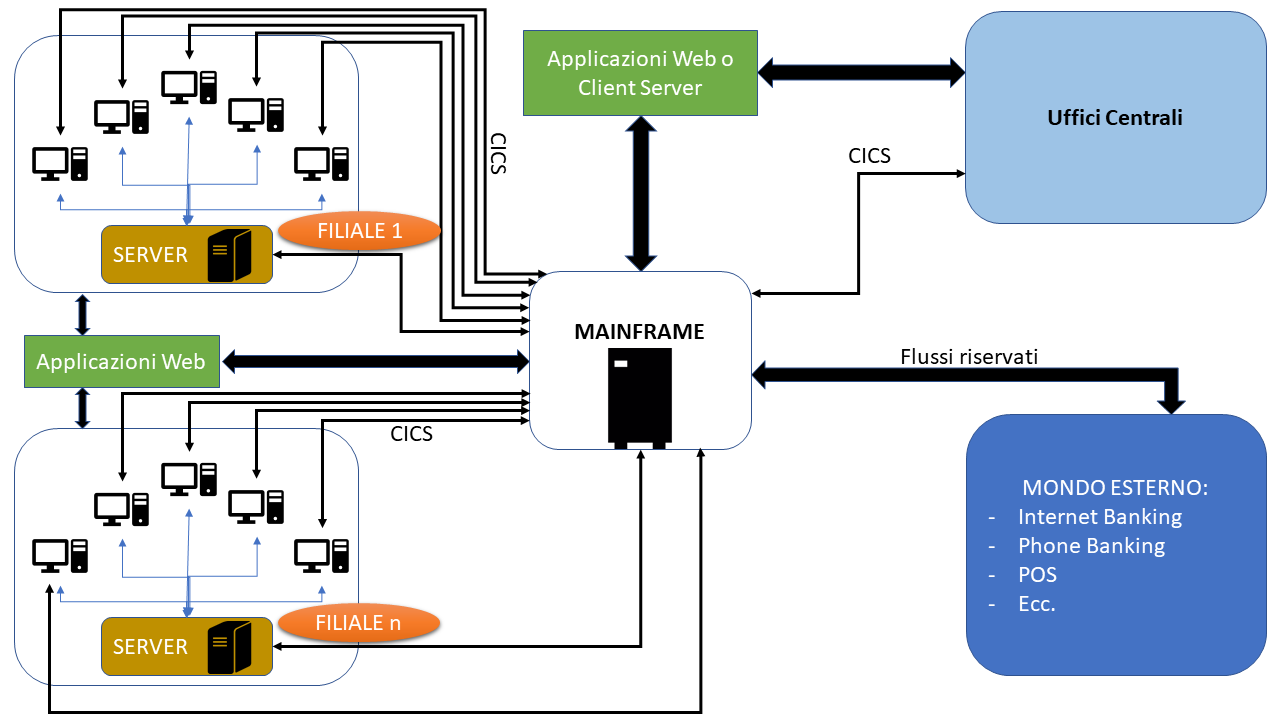
\includegraphics[width=1\textwidth]{immagini/Architettura}
	   	\caption{Architettura della piattaforma Host}
	\end{figure}

	
\subsubsection{COBOL}
In questa sotto sottosezione riporterò i concetti fondamentali di quello che è il linguaggio di programmazione COBOL e l'uso che se ne fa, riportando poi alcuni esempio dei formalismi principali tramite i quali i moduli delle applicazioni host elaborano i dati.
	
\subsubsection{JCL}
In questa sotto sottosezione riporterò i concetti fondamentali di quello che è il linguaggio di scripting JCL e riportando qualche esempio dell'uso che se ne fa, ovvero il controllo dell'esecuzione di moduli COBOL.

\section{Processo di sviluppo}
In questo inizio di sezione introdurrò la fase di stage relativa al processo di sviluppo del progetto di stage.

\subsection{Analisi dei requisiti}
In questa sottosezione descriverò l'attività di analisi dei requisiti e riporterò il modo in cui è stata svolta.

\subsection{Progettazione}
In questa sottosezione descriverò l'attività di progettazione delle implementazioni richieste per lo svolgimento del progetto di stage.
		
\subsection{Codifica}
In questa sottosezione descriverò l'attività di codifica delle implementazioni richieste per lo svolgimento del progetto di stage.
	
\section{Verifica e validazione}
In questa sezione descriverò le attività di Verifica e Validazione delle implementazioni richieste per lo svolgimento del progetto di stage, in particolare descriverò singolarmente l'analisi statica e dinamica effettuata a questo fine.

\subsection{Analisi statica}
In questa sottosezione parlerò degli strumenti utilizzati per l'analisi statica del codice prodotto.
	
\subsection{Analisi dinamica}
In questa sottosezione parlerò dei metodi utilizzati per l'analisi dinamica che utilizza la divisione.

\subsection{Collaudo}
In questa sottosezione parlerò dei metodi utilizzati per il collaudo che utilizza la divisione. Nello specifico parlerò della figura di collaudatore e dei documenti di collaudo che l'azienda proponente richiede ad ogni rilascio.
	
\section{Valutazione del prodotto}
In questa sezione parlerò della valutazione dei documenti e del prodotto dopo i vari test e collaudi.